\documentclass[aspectratio=169]{beamer}
\usepackage[utf8]{inputenc}
\usepackage[T1]{fontenc}
\usepackage{listings}
\usepackage{xcolor}
\usepackage{graphicx}
\usepackage{tikz}
\usetikzlibrary{positioning,shapes,arrows,calc}
\usepackage{amsmath}
\usepackage{booktabs}

% Theme
\usetheme{Madrid}
\usecolortheme{default}

% Custom colors
\definecolor{aspblue}{RGB}{102, 126, 234}
\definecolor{asppurple}{RGB}{118, 75, 162}
\definecolor{codebg}{RGB}{45, 45, 45}
\definecolor{codetext}{RGB}{248, 248, 242}

\setbeamercolor{palette primary}{bg=aspblue,fg=white}
\setbeamercolor{palette secondary}{bg=asppurple,fg=white}
\setbeamercolor{palette tertiary}{bg=aspblue,fg=white}
\setbeamercolor{palette quaternary}{bg=asppurple,fg=white}
\setbeamercolor{structure}{fg=aspblue}
\setbeamercolor{section in toc}{fg=aspblue}

% Code listing style
\lstdefinestyle{asplisting}{
    backgroundcolor=\color{codebg},
    basicstyle=\ttfamily\footnotesize\color{codetext},
    keywordstyle=\color{orange},
    commentstyle=\color{green!60},
    stringstyle=\color{red!60},
    numbers=none,
    breaklines=true,
    frame=single,
    rulecolor=\color{aspblue},
    xleftmargin=5pt,
    xrightmargin=5pt,
    showstringspaces=false,
    tabsize=2
}

\lstset{style=asplisting}

% Title page information
\title[ASP goes to School]{Answer Set Programming goes to School}
\subtitle{Can High School Students Learn Declarative Programming?}
\author[Dennison, Dietz \& Philipp]{%
    Racquel Dennison\inst{1} \and
    Emmanuelle Dietz\inst{2} \and
    Hanna Philipp\inst{3}
}
\institute{
    \inst{1} University of Cape Town and CAIR, South Africa \\
    \inst{2} Airbus Central Research \& Technology, Hamburg, Germany \\
    \inst{3} Weißeritzgymnasium Freital, Freital, Germany
}
\date{\today}

\begin{document}

% Slide 1: Title
\begin{frame}
    \titlepage
\end{frame}

% Slide 2: Research Question & Motivation
\begin{frame}{Research Question}
    \framesubtitle{Is ASP suitable for learning at high school level?}

    Human reasoning is \textbf{non-monotonic}~\cite{byrne:89} \\
    $\Rightarrow$ Classical logic inadequate \\
    $\Rightarrow$ ASP rooted in non-monotonic logics~\cite{BrewkaEiterTruszczynski11,GebserKaufmannSchaub12a}

    \vspace{0.8cm}

    \Large \textbf{Can a high school student learn and apply ASP?}

    \vspace{0.8cm}

    \normalsize
    \textbf{Approach:} A high school student solves their school's classroom scheduling problem

    \vspace{0.5cm}

    \begin{columns}[c]
        \begin{column}{0.48\textwidth}
            \centering
            \textbf{Why ASP?}
            \begin{itemize}
                \item Declarative thinking
                \item Proven for scheduling~\cite{teaspoon:2019,lunch_2023}
                \item But is it \emph{learnable}?
            \end{itemize}
        \end{column}
        \begin{column}{0.48\textwidth}
            \centering
            \textbf{Why This Matters?}
            \begin{itemize}
                \item Different paradigm
                \item Real-world problems
                \item Early CS education
            \end{itemize}
        \end{column}
    \end{columns}
\end{frame}

% Slide 3: The Problem - Visual
\begin{frame}{The School Scheduling Problem}
    \framesubtitle{Weißeritzgymnasium Freital}

    \textbf{Assign:} Classes $\rightarrow$ Rooms + Teachers + Time slots

    \vspace{0.5cm}

    \begin{columns}[c]
        \begin{column}{0.3\textwidth}
            \centering
            \tikz[scale=0.8]{
                \draw[fill=aspblue!30] (0,0) rectangle (2,1.5) node[pos=.5] {36 Teachers};
                \draw[fill=asppurple!30] (0,1.7) rectangle (2,3.2) node[pos=.5] {19 Subjects};
            }
        \end{column}
        \begin{column}{0.35\textwidth}
            \centering
            \tikz[scale=0.8]{
                \foreach \floor in {0,...,4} {
                    \draw[fill=aspblue!20] (0,\floor*0.6) rectangle (3,\floor*0.6+0.5);
                    \node at (1.5,\floor*0.6+0.25) {\tiny Floor \floor};
                }
                \node[below] at (1.5,-0.3) {$\sim$37 Rooms};
            }
        \end{column}
        \begin{column}{0.3\textwidth}
            \centering
            \tikz[scale=0.65]{
                \foreach \x in {0,...,4} {
                    \ifnum\x=0 \node at (\x*0.8, 3.5) {\tiny Mo};\fi
                    \ifnum\x=1 \node at (\x*0.8, 3.5) {\tiny Di};\fi
                    \ifnum\x=2 \node at (\x*0.8, 3.5) {\tiny Mi};\fi
                    \ifnum\x=3 \node at (\x*0.8, 3.5) {\tiny Do};\fi
                    \ifnum\x=4 \node at (\x*0.8, 3.5) {\tiny Fr};\fi
                    \foreach \y in {0,...,5} {
                        \draw[fill=asppurple!20] (\x*0.8,\y*0.45) rectangle (\x*0.8+0.7,\y*0.45+0.4);
                    }
                }
                \node[below] at (1.6,-0.3) {\small 30 Slots};
            }
        \end{column}
    \end{columns}

    \vspace{0.7cm}

    \textbf{Constraints:} No double-booking • Specialized rooms • Block hours (max 2 consecutive)

    \vspace{0.3cm}

    \textbf{Optimize:} Minimize distances • Maximize blocks • Teacher work-life balance
\end{frame}

% Slide 4: Example Schedule Slot
\begin{frame}{Example: One Time Slot}

    \textbf{Monday, 10:00 AM (Slot 3)}

    \vspace{0.5cm}

    \vspace{0.1cm}

    \centering
    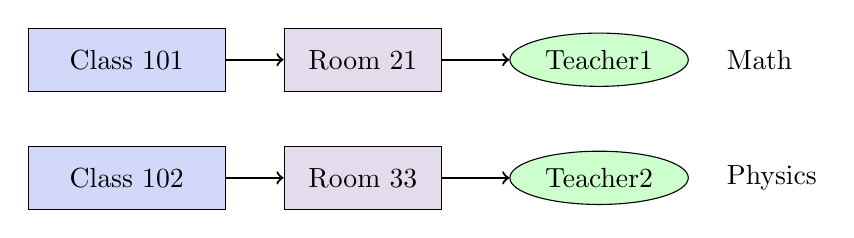
\begin{tikzpicture}[
        class/.style={rectangle, draw, fill=aspblue!30, minimum width=2.5cm, minimum height=0.8cm},
        room/.style={rectangle, draw, fill=asppurple!20, minimum width=2cm, minimum height=0.8cm},
        teacher/.style={ellipse, draw, fill=green!20, minimum width=2cm, minimum height=0.6cm}
    ]
        % Class 101
        \node[class] (c101) at (0,2) {Class 101};
        \node[room] (r21) at (3,2) {Room 21};
        \node[teacher] (t1) at (6,2) {Teacher1};
        \node[right] at (7.5,2) {Math};

        \draw[->, thick] (c101) -- (r21);
        \draw[->, thick] (r21) -- (t1);

        % Class 102
        \node[class] (c102) at (0,0.5) {Class 102};
        \node[room] (r33) at (3,0.5) {Room 33};
        \node[teacher] (t2) at (6,0.5) {Teacher2};
        \node[right] at (7.5,0.5) {Physics};

        \draw[->, thick] (c102) -- (r33);
        \draw[->, thick] (r33) -- (t2);
    \end{tikzpicture}

    \vspace{0.5cm}

    \textbf{Question:} How to encode this in ASP?
\end{frame}

% Slide 5: Facts
\begin{frame}[fragile]{ASP Encoding: Facts}
    \framesubtitle{Student Feedback: "Writing facts is easy"}

    \textbf{Ground truth - what we know:}

    \begin{lstlisting}[language=Prolog]
% Teachers and their qualifications
teacher(teacher1, ma).
teacher(teacher1, info).
teacher(teacher2, ph).

% Rooms with coordinates (ID, X, Y, Floor)
room(21, 0, 0, 2).
room(33, 2, 0, 3).

% Curriculum: Class needs X hours of subject F
curriculum(101, ma, 4).
curriculum(102, ph, 2).

% Specialized rooms
room_subject(33, ph).   % Room 33 for physics only
    \end{lstlisting}

    \vspace{0.2cm}
    \textbf{Challenge:} Determining optimal structure - what information to include?
\end{frame}

% Slide 6: Standard Rules
\begin{frame}[fragile]{ASP Encoding: Standard Rules}
    \framesubtitle{Student Feedback: "Intuitive once an example is provided"}

    \textbf{Derive new information from facts:}

    \begin{lstlisting}[language=Prolog]
% Calculate distance between rooms (Manhattan + floor penalty)
dist_x(R,R1,DX) :- room(R,X,_,_), room(R1,X1,_,_),
                   X>=X1, DX=X-X1.

dist(R,R1,D) :- dist_x(R,R1,DX), dist_y(R,R1,DY),
                dist_z(R,R1,DZ),
                D = DX + DY + DZ*4.    % Floor changes cost 4x
    \end{lstlisting}

    \vspace{0.5cm}

    \textbf{Example:} Room 21 (0,0,2) to Room 33 (2,0,3)
    \begin{align*}
        \text{Distance} &= |0-2| + |0-0| + |2-3| \times 4 = 2 + 0 + 4 = \textbf{6 units}
    \end{align*}

    \textbf{Learning:} Initial encoding didn't capture all edge cases
\end{frame}

% Slide 7: Choice Rules
\begin{frame}[fragile]{ASP Encoding: Choice Rules}
    \framesubtitle{Student Feedback: "More difficult - managing bounds is tricky"}

    \textbf{Let the solver decide - generate possible schedules:}

    \begin{lstlisting}[language=Prolog]
2{allocation(K,R,F,T,S,L): teacher(L,F),
                           room_subject(R,F),
                           week(T,S)}2
  :- curriculum(K, F, X), X=2.
    \end{lstlisting}

    \vspace{0.5cm}

    \textbf{Meaning:} Choose exactly \textbf{2 allocations} for class K and subject F when curriculum requires 2 hours

    \vspace{0.5cm}

    \textbf{Example result:}
    \begin{lstlisting}[language=Prolog]
allocation(102, 33, ph, mo, 3, teacher2).    % Monday slot 3
allocation(102, 33, ph, mi, 2, teacher2).    % Wednesday slot 2
    \end{lstlisting}

    \textbf{Challenge:} Understanding min/max bounds and rule head structure
\end{frame}

% Slide 8: Integrity Constraints
\begin{frame}[fragile]{ASP Encoding: Integrity Constraints}
    \framesubtitle{Student Feedback: "More accessible than choice rules"}

    \textbf{Eliminate invalid solutions:}

    \begin{lstlisting}[language=Prolog]
% Teacher cannot teach two classes simultaneously
:- allocation(K1, _, _, T, S, L),
   allocation(K2, _, _, T, S, L),
   K1 != K2.
    \end{lstlisting}

    \vspace{0.5cm}

    \vspace{0.1cm}

    \centering
    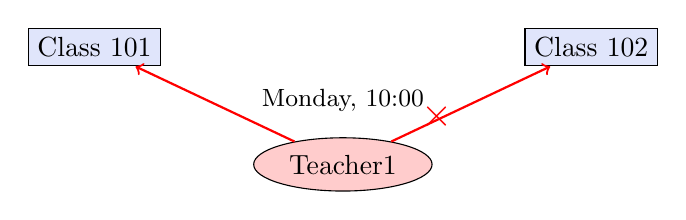
\begin{tikzpicture}[scale=0.9]
        \node[ellipse, draw, fill=red!20, minimum width=2cm] (teacher) {Teacher1};
        \node[rectangle, draw, fill=aspblue!20, above left=1cm and 1.5cm of teacher] (k1) {Class 101};
        \node[rectangle, draw, fill=aspblue!20, above right=1cm and 1.5cm of teacher] (k2) {Class 102};
        \node[above=0.2cm of teacher] {\small Monday, 10:00};

        \draw[->, thick, red] (teacher) -- (k1);
        \draw[->, thick, red] (teacher) -- (k2);
        \node[above right=0.1cm of teacher, red, font=\Large\bfseries] {$\times$};
    \end{tikzpicture}

    \vspace{0.3cm}
    \textbf{Why easier?} Behavior similar to standard rules - just negation!
\end{frame}

% Slide 9: Aggregates
\begin{frame}[fragile]{ASP Encoding: Aggregates}
    \framesubtitle{Student Feedback: "Initially confusing - which variables?"}

    \textbf{Count or sum over multiple solutions:}

    \begin{lstlisting}[language=Prolog]
% Teacher should have at least 1 day off (home office)
:- teacher(L, F),
   #count{T, S : allocation(K, R, F, T, S, L)} > 4.
    \end{lstlisting}

    \vspace{0.3cm}

    \textbf{Common mistake:} Forgot grounding predicate \texttt{teacher(L, F)}!

    \vspace{0.5cm}

    \begin{lstlisting}[language=Prolog]
% Calculate total travel distance
travel_cost(K, D, T, S) :-
    allocation(K, R1, _, T, S1, _),
    allocation(K, R, _, T, S, _),
    dist(R1, R, D), S1 = S+1.

total_distance(K, G) :-
    #sum{D,T,S : travel_cost(K,D,T,S)} = G, class(K).
    \end{lstlisting}

    \textbf{Challenge:} Determining which variables are relevant in the aggregate
\end{frame}

% Slide 10: Optimization
\begin{frame}[fragile]{ASP Encoding: Optimization}
    \framesubtitle{Student Feedback: "Simpler than aggregates"}

    \textbf{Multi-objective optimization:}

    \begin{lstlisting}[language=Prolog]
% Minimize student travel
#minimize{G,K : total_distance(K,G)}.

% Maximize teaching blocks (consecutive hours)
block(F, S, S1, T, K, L) :-
    allocation(K, R, F, T, S, L),
    allocation(K, R, F, T, S1, L),
    S1 = S+1, S != 6.

sum_blocks(B) :- #sum{S,F,S1,T,K,L : block(F,S,S1,T,K,L)} = B.
#maximize{B : sum_blocks(B)}.
    \end{lstlisting}

    \vspace{0.5cm}

    \textbf{Conflicting objectives} $\rightarrow$ Pareto front analysis

    \vspace{0.3cm}

    \centering
    \small Fewer variable constructs make optimization statements easier to understand
\end{frame}

% Slide 11: Learning Experience
\begin{frame}{Learning Experience Summary}

    \begin{columns}[c]
        \begin{column}{0.48\textwidth}
            \textbf{What was EASY:}
            \begin{itemize}
                \item[\textcolor{green}{\checkmark}] Writing facts
                \item[\textcolor{green}{\checkmark}] Standard rules (with examples)
                \item[\textcolor{green}{\checkmark}] Integrity constraints
                \item[\textcolor{green}{\checkmark}] Immediate solver feedback
            \end{itemize}
        \end{column}
        \begin{column}{0.48\textwidth}
            \textbf{What was HARD:}
            \begin{itemize}
                \item[\textcolor{red}{!}] Choice rule bounds
                \item[\textcolor{red}{!}] Aggregates (variables)
                \item[\textcolor{red}{!}] Covering edge cases
                \item[\textcolor{red}{!}] Fact structure design
            \end{itemize}
        \end{column}
    \end{columns}

    \vspace{0.7cm}

    \centering
    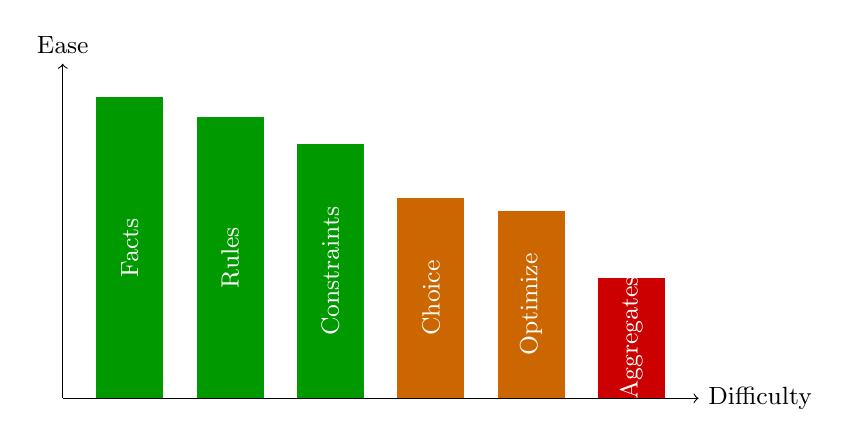
\begin{tikzpicture}[scale=0.85]
        % Bars
        \fill[green!60!black] (0.5,0) rectangle (1.5,4.5) node[pos=.5, rotate=90, white, font=\small] {Facts};
        \fill[green!60!black] (2,0) rectangle (3,4.2) node[pos=.5, rotate=90, white, font=\small] {Rules};
        \fill[green!60!black] (3.5,0) rectangle (4.5,3.8) node[pos=.5, rotate=90, white, font=\small] {Constraints};
        \fill[orange!80!black] (5,0) rectangle (6,3.0) node[pos=.5, rotate=90, white, font=\small] {Choice};
        \fill[orange!80!black] (6.5,0) rectangle (7.5,2.8) node[pos=.5, rotate=90, white, font=\small] {Optimize};
        \fill[red!80!black] (8,0) rectangle (9,1.8) node[pos=.5, rotate=90, white, font=\small] {Aggregates};

        % Axis
        \draw[->] (0,0) -- (9.5,0) node[right, font=\small] {Difficulty};
        \draw[->] (0,0) -- (0,5) node[above, font=\small] {Ease};
    \end{tikzpicture}

    \vspace{0.3cm}
    \textbf{Key Insight:} \emph{Examples} and \emph{iterative feedback} overcome most difficulties!
\end{frame}

% Slide 12: Implementation & Results
\begin{frame}{Implementation \& Results}

    \textbf{System:} Python + Clingo + Pandas

    \vspace{0.5cm}

    \vspace{0.1cm}

    \centering
    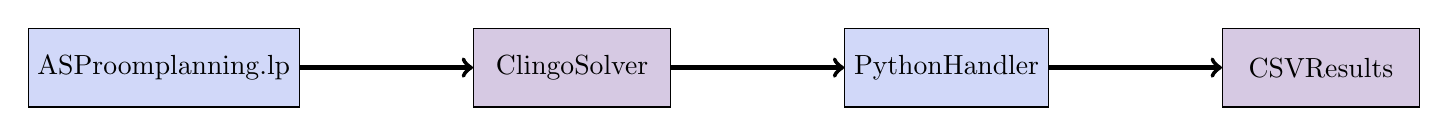
\begin{tikzpicture}[node distance=2.2cm]
        \node[rectangle, draw, fill=aspblue!30, minimum width=2.5cm, minimum height=1cm] (asp) {ASP\\roomplanning.lp};
        \node[rectangle, draw, fill=asppurple!30, minimum width=2.5cm, minimum height=1cm, right=of asp] (clingo) {Clingo\\Solver};
        \node[rectangle, draw, fill=aspblue!30, minimum width=2.5cm, minimum height=1cm, right=of clingo] (python) {Python\\Handler};
        \node[rectangle, draw, fill=asppurple!30, minimum width=2.5cm, minimum height=1cm, right=of python] (output) {CSV\\Results};

        \draw[->, ultra thick] (asp) -- (clingo);
        \draw[->, ultra thick] (clingo) -- (python);
        \draw[->, ultra thick] (python) -- (output);
    \end{tikzpicture}

    \vspace{0.7cm}

    \begin{columns}[c]
        \begin{column}{0.48\textwidth}
            \textbf{Execution:}
            \begin{itemize}
                \item Grounding: minutes
                \item Solving: varies
                \item Optimal found: \checkmark
            \end{itemize}
        \end{column}
        \begin{column}{0.48\textwidth}
            \textbf{Output:}
            \begin{itemize}
                \item Full schedule (CSV)
                \item Distance metrics
                \item Multi-objective costs
            \end{itemize}
        \end{column}
    \end{columns}

    \vspace{0.5cm}

    \vspace{0.1cm}

    \centering
    \textbf{Result:} Generated schedules are \emph{actually usable} by the school!
\end{frame}

% Slide 13: Related Work
\begin{frame}{Related Work}

    \textbf{ASP for Scheduling:}

    \vspace{0.5cm}

    \begin{tabular}{lll}
        \toprule
        \textbf{System} & \textbf{Domain} & \textbf{Reference} \\
        \midrule
        teaspoon & University timetabling & \cite{teaspoon:2019} \\
        LUNCH & Course scheduling & \cite{lunch_2023} \\
        Nurse scheduling & Hospital shifts & \cite{Nabeshima_2026} \\
        Chemotherapy & Treatment planning & \cite{DODARO_GALATA_GRIONI_MARATEA_MOCHI_PORRO_2021} \\
        \bottomrule
    \end{tabular}

    \vspace{0.8cm}

    \Large \textbf{Our Contribution:}

    \vspace{0.3cm}

    \normalsize
    First study evaluating ASP from a \textbf{high school student's learning perspective}, \\
    not just as a solving tool.
\end{frame}

% Slide 14: Conclusions
\begin{frame}{Conclusions}

    \LARGE \textbf{Can high school students learn ASP?}

    \vspace{0.5cm}

    \Large \textcolor{green!60!black}{YES!} \normalsize (with caveats)

    \vspace{0.7cm}

    \begin{enumerate}
        \item \textbf{Declarative thinking is learnable}
        \begin{itemize}
            \item Clear separation: facts vs. decisions
            \item Logical structure is intuitive
        \end{itemize}

        \vspace{0.3cm}

        \item \textbf{Learning curve exists}
        \begin{itemize}
            \item Facts, rules, constraints: accessible
            \item Aggregates: challenging (needs careful teaching)
        \end{itemize}

        \vspace{0.3cm}

        \item \textbf{Examples + feedback = key to success}
        \begin{itemize}
            \item Iterative development crucial
            \item Real problems motivate learning
        \end{itemize}
    \end{enumerate}

    \vspace{0.5cm}

    \vspace{0.1cm}

    \centering
    \textbf{ASP education can start earlier than we thought!}
\end{frame}

% Slide 15: Questions
\begin{frame}[plain]
    \centering
    \vspace{2cm}

    \Huge \textbf{Questions?}

    \vspace{1.5cm}

    \Large Thank you for your attention!

    \vspace{1cm}

    \normalsize
    Racquel Dennison, Emmanuelle Dietz, Hanna Philipp

    \vspace{0.5cm}

    \small
    \texttt{Answer Set Programming goes to School}
\end{frame}

% References
\begin{frame}[allowframebreaks]{References}
    \footnotesize
    \begin{thebibliography}{99}

    \bibitem{byrne:89}
    R.~M.~J.~Byrne.
    \newblock Suppressing valid inferences with conditionals.
    \newblock {\em Journal of Memory and Language}, 31:61--83, 1989.

    \bibitem{BrewkaEiterTruszczynski11}
    G.~Brewka, T.~Eiter, and M.~Truszczyński.
    \newblock Answer set programming at a glance.
    \newblock {\em Communications of the ACM}, 54(12):92--103, 2011.

    \bibitem{GebserKaufmannSchaub12a}
    M.~Gebser, B.~Kaufmann, and T.~Schaub.
    \newblock Conflict-Driven Answer Set Solving: From Theory to Practice.
    \newblock {\em Artificial Intelligence}, 187--188, 2012.

    \bibitem{teaspoon:2019}
    M.~Banbara et al.
    \newblock teaspoon: solving the curriculum-based course timetabling problems with ASP.
    \newblock {\em Annals of Operations Research}, 275(1):3--37, 2019.

    \bibitem{lunch_2023}
    A.~Lima et al.
    \newblock LUNCH: an Answer Set Programming System for Course Scheduling.
    \newblock {\em ENIAC}, 2023.

    \bibitem{Nabeshima_2026}
    H.~Nabeshima, M.~Banbara, T.~Schaub, and T.~Soh.
    \newblock The ASP-based Nurse Scheduling System.
    \newblock {\em EPTCS}, 439:334--348, 2026.

    \bibitem{DODARO_GALATA_GRIONI_MARATEA_MOCHI_PORRO_2021}
    C.~Dodaro et al.
    \newblock An ASP-based Solution to Chemotherapy Treatment Scheduling.
    \newblock {\em TPLP}, 21(6):835--851, 2021.

    \end{thebibliography}
\end{frame}

\end{document}
